软件仿真具体情况如下:

\begin{itemize}
\item 仿真平台:ModelSim-Altera 10.4b
\item 输入序列:[1, 0, 0, 1, 0, 0, 0, 0, 1, 0, 1, 1, 0, 0]
\item 编码方式:(2,1,3)卷积码
\item 调制方式:QPSK
\item 是否交织:是
\item 是否加噪声:是
\end{itemize}

编码输入及输出波形已在原理部分有所展示,在此不予赘述。我们将考虑的内容包括:(1)通过噪声信道前后发送序列;(2)编码后序列与解码输入;(3)解码后序列与原始序列。\\

\noindent {\bf \large 通过噪声信道前后发送序列}

通过噪声信道前序列即交织后序列,记作bit\_send。而通过噪声信道后的序列记作bit\_recv。如.\ref{fig:BitSig} 中所示,由于交织需要一定的缓冲,从而两个信号之间存在延迟。仔细观察可以看出,这两个序列存在一些差异,这是由于我们添加的噪声较大,正好用来检验卷积码的纠错能力。
\begin{figure}[htb]
\centering
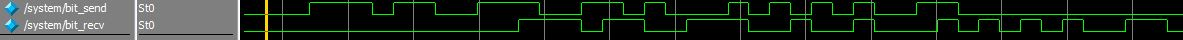
\includegraphics[width=1.2\textwidth]{images//BitSig.jpg}
\caption{\label{fig:BitSig}通过噪声信道前后序列}
\end{figure}\\

\noindent {\bf \large 编码后序列与解码输入}

编码后序列及code\_send,而解码输入记作code\_recv,分别如图.\ref{fig:CodeSend},图.\ref{fig:CodeRecv}所示。同样的,由于信道噪声较强,二者并不一样。
\begin{figure}[htb]
\centering
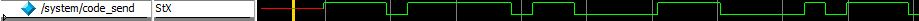
\includegraphics[width=1.2\textwidth]{images//CodeSend.jpg}
\caption{\label{fig:CodeSend}编码后序列}
\end{figure}
\begin{figure}[htb]
\centering
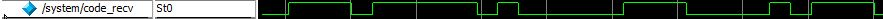
\includegraphics[width=1.2\textwidth]{images//CodeRecv.jpg}
\caption{\label{fig:CodeRecv}解码输入序列}
\end{figure}\\

\noindent {\bf \large 解码后序列与原始序列}

解码后序列记为data\_recv, 如图.\ref{fig:DataRecv}所示,和输入序列完全相同,体现了卷积码的纠错能力。
\begin{figure}[htb]
\centering
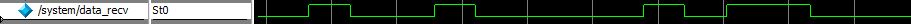
\includegraphics[width=1.2\textwidth]{images//DataRecv.jpg}
\caption{\label{fig:DataRecv}解码后序列}
\end{figure}
我们还可以观察一下Viterbi算法给出的最大似然输入,记作code\_prob,如如图.\ref{fig:CodeProb}所示,和code\_send完全相同。
\begin{figure}[htb]
\centering
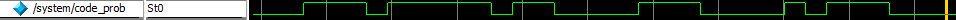
\includegraphics[width=1.2\textwidth]{images//CodeProb.jpg}
\caption{\label{fig:CodeProb}最大似然输入}
\end{figure}

单独看起来,每个模块都不算复杂,无非是对输入数据做一些处理。但当我们试图把这些模块组合成一个系统是,同步成了最为关键的问题。举例来说,对于交织模块,如果我们交织的部分和实际输入存在1bit偏差,这样相当于在编码后结果前加一位0,并减去末尾一比特。这对于卷积码来说是灾难性的错误,我们将不可能恢复出正确的序列。
为了解决同步的问题,我们为每个模块都设置了同步信号。只有当下一级模块收到上一级模块的有效同步信号时,才开始进行相关的操作。牺牲一部分延时性能来换取同步的准确性。

